% LAST UPDATED 24 JUNE 2022

\documentclass{beamer}
\usetheme{Pittsburgh}
\usecolortheme{default}

% PACKAGES USED
\usepackage{physics}
\usepackage{amsthm}
\usepackage{braket}
\usepackage[super]{nth}
% MACROS

%% ENVIROMENTS
\newtheorem{remark}{Remark}
\setbeamercolor{block title}{use=structure,fg=white,bg=structure.fg!75!black}
\setbeamercolor{block body}{parent=normal text,use=block title,bg=block title.bg!10!bg}
%% COMMANDS
\newcommand{\dcp}{\delta_{CP}}
\renewcommand\bra[1]{{\langle{#1}|}}
\makeatletter
\renewcommand\ket[1]{%
  \@ifnextchar\bra{\k@t{#1}\!}{\k@t{#1}}%
}
\newcommand\k@t[1]{{|{#1}\rangle}}
\DeclareMathAlphabet\mathbfcal{OMS}{cmsy}{b}{n}
\makeatother

% TOC
\AtBeginSection[]
{
  \begin{frame}
    \frametitle{Table of Contents}
    \tableofcontents[currentsection]
  \end{frame}
}

%Information to be included in the title page:
\title[ACRONYM] %optional
{QCVN Group Meeting}
\subtitle{Haar measure \& Unitary t-design\\-- Towards URB for qutrit}

\author[] % (optional, for multiple authors)
{Dinh-Tien Nguyen}
\institute[] % (optional)
{
Faculty of Physics\\
VNU University of Science
}
\date{}

\begin{document}
\frame{\titlepage}
\tableofcontents
\section{Unitary randomized benchmarking}
\begin{frame}
  \frametitle{Complete protocol of URB}
  A standard unitary randomized benchmarking consists of 
  \begin{enumerate}
    \item Generate RB sequences
    \begin{align} 
      \mathcal{S}_{i_m}=\bigodot_{j=1}^{m+1}(\Lambda_{i_j,j}\odot C_{i_j})
    \end{align}
    \item For each sequence, calculate survival probability
    \begin{align}
      \Tr[E_\psi\mathcal{S}_{i_m}(\rho_\psi)]
    \end{align}
    \item Average over random realizations to find the \textit{average} fidelity
    \begin{align} 
      F_{seq}(m,\psi) = \Tr\left(E_\psi \mathcal{S}_m(\rho_\psi)\right)
    \end{align}
    \item Fit the results to the model of exponential decay.
  \end{enumerate}
\end{frame}
\subsection{Generate RB sequences}
\begin{frame}
  \frametitle{Generate RB sequences}
  \begin{definition}
    A sequence of $m+1$ quantum operations with the first $m$ operations chosen \textit{uniformly} at random from some group $\mathcal{G}\in U(d)$ and the final operation $(m+1)$ chosen so that the net sequence is the identity operation.
  \end{definition}
  \begin{itemize}
    \item We primarily focus on $C_3\in U(3^n)$, because they can be realized efficiently on both quantum \& classical hardware.
    \item For each length $m$, we choose $K_m$ RB sequences. Each sequence contains $m$ \textit{random} element $C_{i_j}$ \textit{sampled uniformly} from $C_3$.
    \item The $C_{i_{m+1}}$ element is defined as $(C_{i_1}\cdot\cdots C_{i_m})^{-1}$.
  \end{itemize}
\end{frame}
\subsection{Measure survival probability \& fit results}
\begin{frame}
  \frametitle{Measure survival probability}
  The survival probability is defined by 
  \begin{align} 
    \Tr[E_\psi\mathcal{S}_{i_m}(\rho_\psi)]
  \end{align}
  where $\rho_\psi$ is the initial state (SPAM absorbed) and $E_\psi$ is the POVM element (having off-diagonal non-zero entries). If noise-free, $$\rho_\psi=E_\psi=|\psi\rangle\langle\psi|$$
  In practice, survival probabilities are probabilities that the qutrit go back to the ground state $\ket{0}$. For example, in the noise-free situation,
  \begin{align} 
    \Tr[E_\psi\mathcal{S}_{i_m}(\rho_\psi)]= p(0)
  \end{align}
\end{frame}
\begin{frame}
  \frametitle{Measure survival probability}
  \begin{theorem}
    The survival probability of the qutrit is the probability we obtain the initial state (or ground state if we prepare $\ket{0}$).
  \end{theorem}
    \textit{Proof.} Suppose we prepare a statistical ensemble $\rho$, taking into account the SPAM error. Then the evolution of such system is governed by
    \begin{align} 
      \rho_\psi \to \sum_i p_i U\ket{\psi_i}\bra{\psi_i}U^\dagger
    \end{align}
  \end{frame}
\begin{frame} 
    The probability of getting result $m$ is 
    \begin{align}
      p(m) &= \sum_i p(m|i)p_i\\
      &=\sum_i \bra{\psi_i} U^\dagger E_{\ket{\psi}} U\ket{\psi_i}p_i\\
      &=\Tr[E_{\ket{\psi}} \sum_i p_i U\ket{\psi_i}\bra{\psi_i}U^\dagger]\\
      &=\Tr[E_{\ket{\psi}}\mathcal{S}_{i_m}(\rho_\psi)]
    \end{align}
    If we intended to prepare an initial ground state, then 
    \begin{align} 
      \Tr[E_{\ket{0}}\mathcal{S}_{i_m}(\rho_{\ket{0}})] = p(0)\tag*{\qed} 
    \end{align}
  \end{frame}
\begin{frame}
  \frametitle{Average sequence fidelity and fit results}
  Average over $K_m$ random realizations of the sequence to find the average sequence fidelity 
  \begin{align} 
    F_{seq}(m,\ket{\psi}) &= \Tr[E_\psi S_{K_m}(\rho_{\psi})]\\
    &= \Tr[E_\psi \dfrac{1}{K_m}\sum_{i_m}\mathcal{S}_{i_m}(\rho_{\psi})]
  \end{align}
  Repeat for different values of $m$ and fit the results for the averaged sequence fidelity to the model 
  \begin{align} 
    F^{(0)}(m,\ket{\psi}) = A_0\alpha^m + B_0
  \end{align}
  where $A_0$ and $B_0$ absorb SPAM error. $\alpha$ is called the \textit{Error per Clifford (EPC)}, relating to the average error-rate.
\end{frame}
\begin{frame}
  \frametitle{Results}
  \begin{figure}
    \centering
    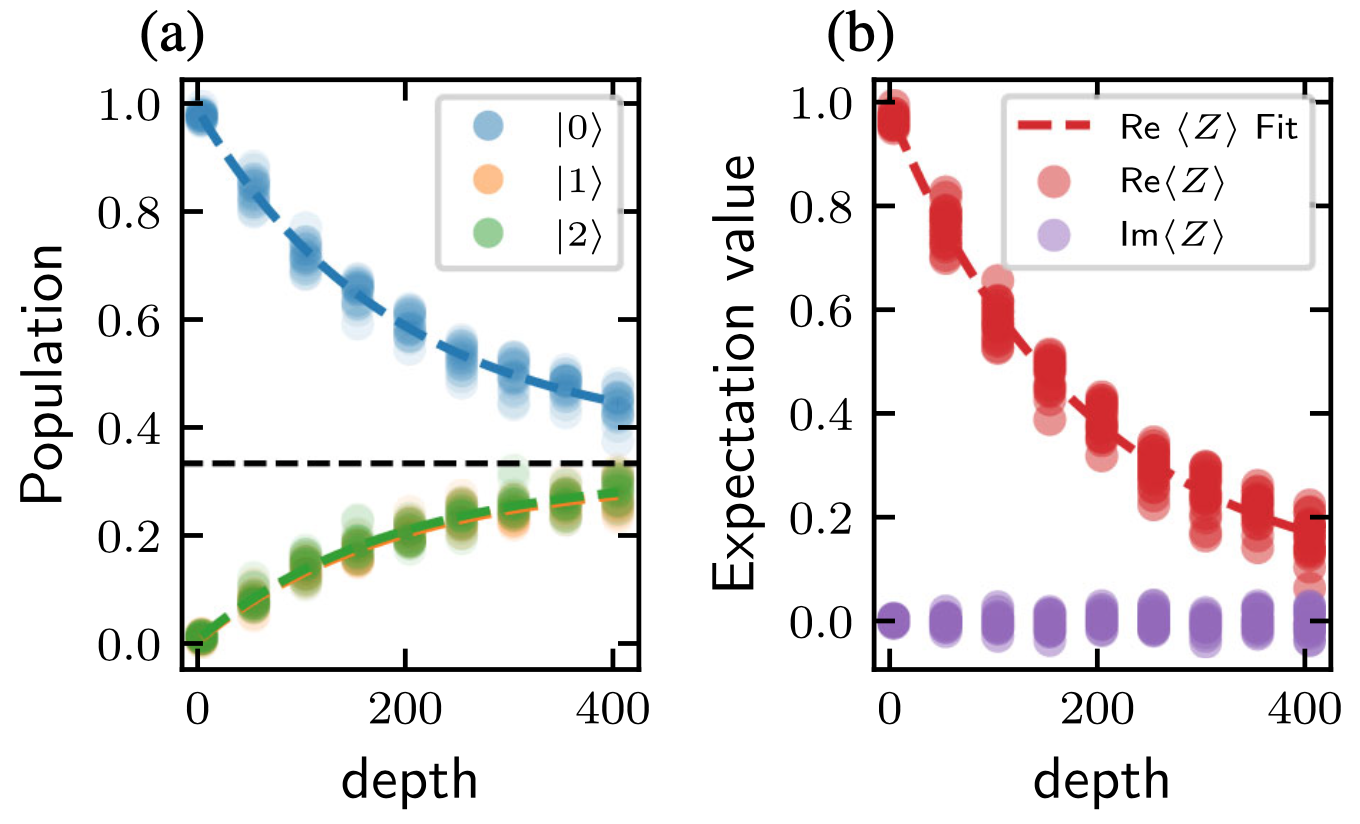
\includegraphics[scale=0.4]{qutrit_urb.png}
    \caption{Qutrit randomized benchmarking [Morvan \textit{et al.} Phys. Rev. Lett.126.210504 (2021)].}
  \end{figure}
\end{frame}
\subsection{Intuition behind URB}
\begin{frame}
  \frametitle{Intuition behind URB}
  \begin{itemize}
    \item By sampling uniformly noisy gates, we create a \textit{depolarizing channel}, characterized by the probability $\alpha$ of the qutrit not being turned into a maximally mixed state $I/3$.
    \item After a sequence of $m$ gates, where the error per gate rate is $\alpha$, then the resulting density matrix is 
    \begin{align} 
      \rho_f^m = \alpha^m \rho_i + (1-\alpha^m)/3\cdot I
    \end{align}
    \item Suppose we start with $\ket{0}$, and the entire sequence is equivalent to the identity operator. The probability of successfully measuring $\ket{0}$ is 
    \begin{align}
      p(0) = \begin{cases}
        \alpha^m[\rho_i]_{00}+1-\alpha/3\\
        \alpha^m+1-\alpha^m/3=2/3\alpha^m + 1/3
      \end{cases}
    \end{align}
  \end{itemize}
\end{frame}
\subsection{Mathematical motivation}
\begin{frame}
  \frametitle{The mathematical theory behind}
  \begin{itemize}
    \item The exponential decay model is not a result of repeating gate in a sequential manner, but \textit{uniformly randomized gates from the Clifford group}. These Clifford gates are noisy, thus $C_{i_j}\odot \Lambda$, where $\Lambda$ constitutes a depolarizing channel. 
    \item Formally speaking, taking an average over a finite group $C_3$ of a quantum channel $\Lambda$ constitutes a twirl.
    \item Twirling over $U(3)$ yeilds exactly the same result as the Clifford group, because the Clifford group $C_3\in U(3)$ is a \textit{unitary 2-design} of the unitary group. 
    \item Buzzing words: \textit{uniformly-randomized}, \textit{unitary t-design}, \textit{twirling over a finite group}.
  \end{itemize}
\end{frame}
\section{Haar measure}
\subsection{The motivation of measure theory}
\begin{frame}
  \frametitle{The motivation of measure theory}
  The theory of random matrices involves extensively the generalised concept of \textit{measure}. 
  \begin{itemize}
    \item In $\mathbb{R}^1, \mathbb{R}^2, \mathbb{R}^3$, think about length, area, and volume.
    \item What about higher dimensions?
    \item What about other spaces?
    \item What about vector spaces, e.g $\mathcal{M}_{3x3}$.
  \end{itemize}
  \begin{definition}[Loosely speaking]
    Measure $\mu$ tells us how mathematical objects (points, matrices, functions, etc.) are distributed in a mathematical set or space--some place is immensily dense, some is not. 
  \end{definition}  
\end{frame}
\begin{frame}
  \frametitle{Example 1: Triple integral of volume $V$}
  \begin{columns}
    \begin{column}{0.4\textwidth}
  \begin{figure}
    \centering
    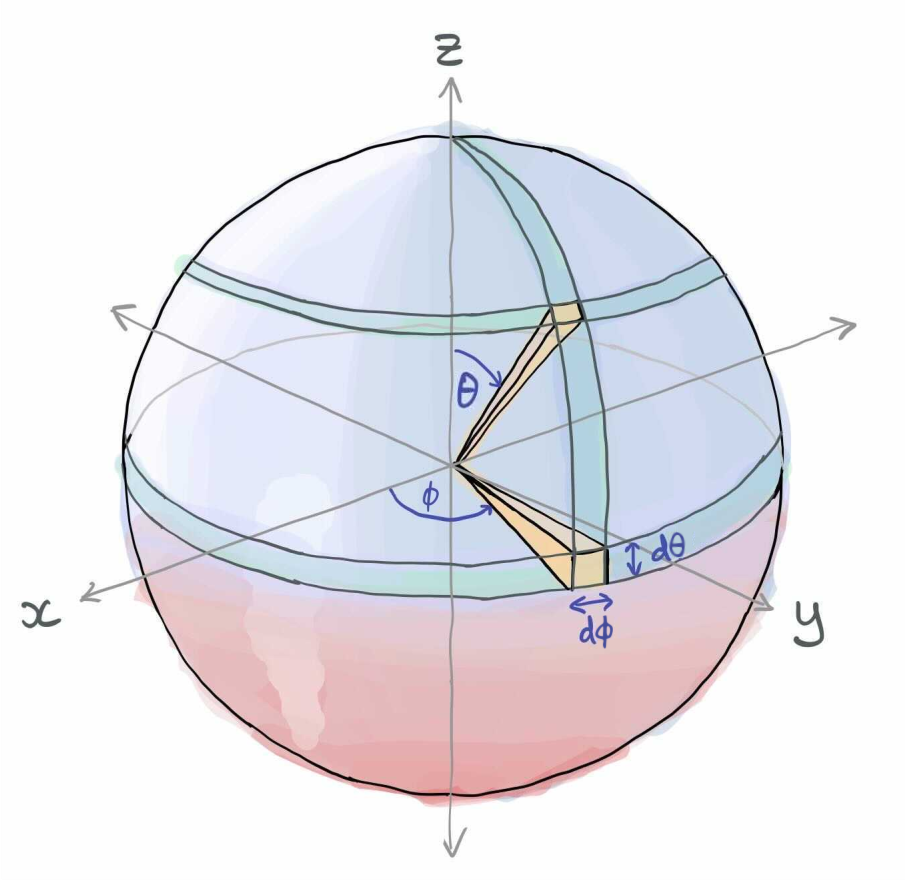
\includegraphics[scale=0.15]{sphere.png}
    \caption{The measure $\mu$ takes into account that these infinitesimal volume is not uniformly distributed over $\mathbb{R}^3$.}
  \end{figure}
\end{column}
\begin{column}{0.6\textwidth}
  The volume of the sphere is \textit{properly measured} when including the measure factor $\mu$
  \begin{align}
    V = \int_0^r\int_0^{2\pi}\int_0^\pi \mu d\rho d\phi d\theta,  
  \end{align}
  where $\mu = \rho^2\sin\theta$ weights portions of the sphere differently depending on where they are in the space.
\end{column}
\end{columns}
\end{frame}
\subsection{The Haar measure}
\begin{frame}
  \frametitle{The Haar measure}
  \begin{itemize}
    \item Similar to points in spherical coordinates uniquely defined by $(\rho, \phi,\theta)$, unitary matrices are uniquely defined by three parameters, e.g $(\theta,\phi,\lambda)$ for every element in $U(2)$.
    \item For every dimension $N$, the unitary matrices of size $N\times N$ constitute the unitary group $U(N)$. Operations on $U(N)$ requires proper measure $\mu$, or the \textit{Haar measure}.
    \item For an $N$-dimensional system, the Haar measure tells us how to weight the elements of $U(N)$. As an example, suppose $f$ is a function acts on $V\in U(N)$, the integral over the group is
    \begin{align} 
      \int_{V\in U(N)} f(V)d\mu_N(V)
    \end{align}
    where the analytical expression of $\mu_N$ is desired.
  \end{itemize}
\end{frame}
\subsection{Haar measure in U(2)}
\begin{frame}
  \frametitle{Haar measure in $U(2)$}
  \begin{problem}[Sampling]
    Given the structure of the group $U(2)$, sample elements of the unitary group $U(2)$ in a properly uniform manner.
  \end{problem}
  \begin{columns}
  \begin{column}{0.6\textwidth}
  \begin{itemize}
    \item The mathematical space we're dealing with is $U(2)$.
    \item The operation is sampling.
    \item An alternative angle of looking: sampling quantum \textit{states} uniformly at random.
    \begin{align} 
      \rho_{\ket{0}} \rightarrow U_{\mu_N}\ket{\psi(\theta,\varphi)}\bra{\psi(\theta,\varphi)}U^\dagger_{\mu_N}
    \end{align}
  \end{itemize}
\end{column}
\begin{column}{0.4\textwidth}
  \begin{figure}
    \centering
    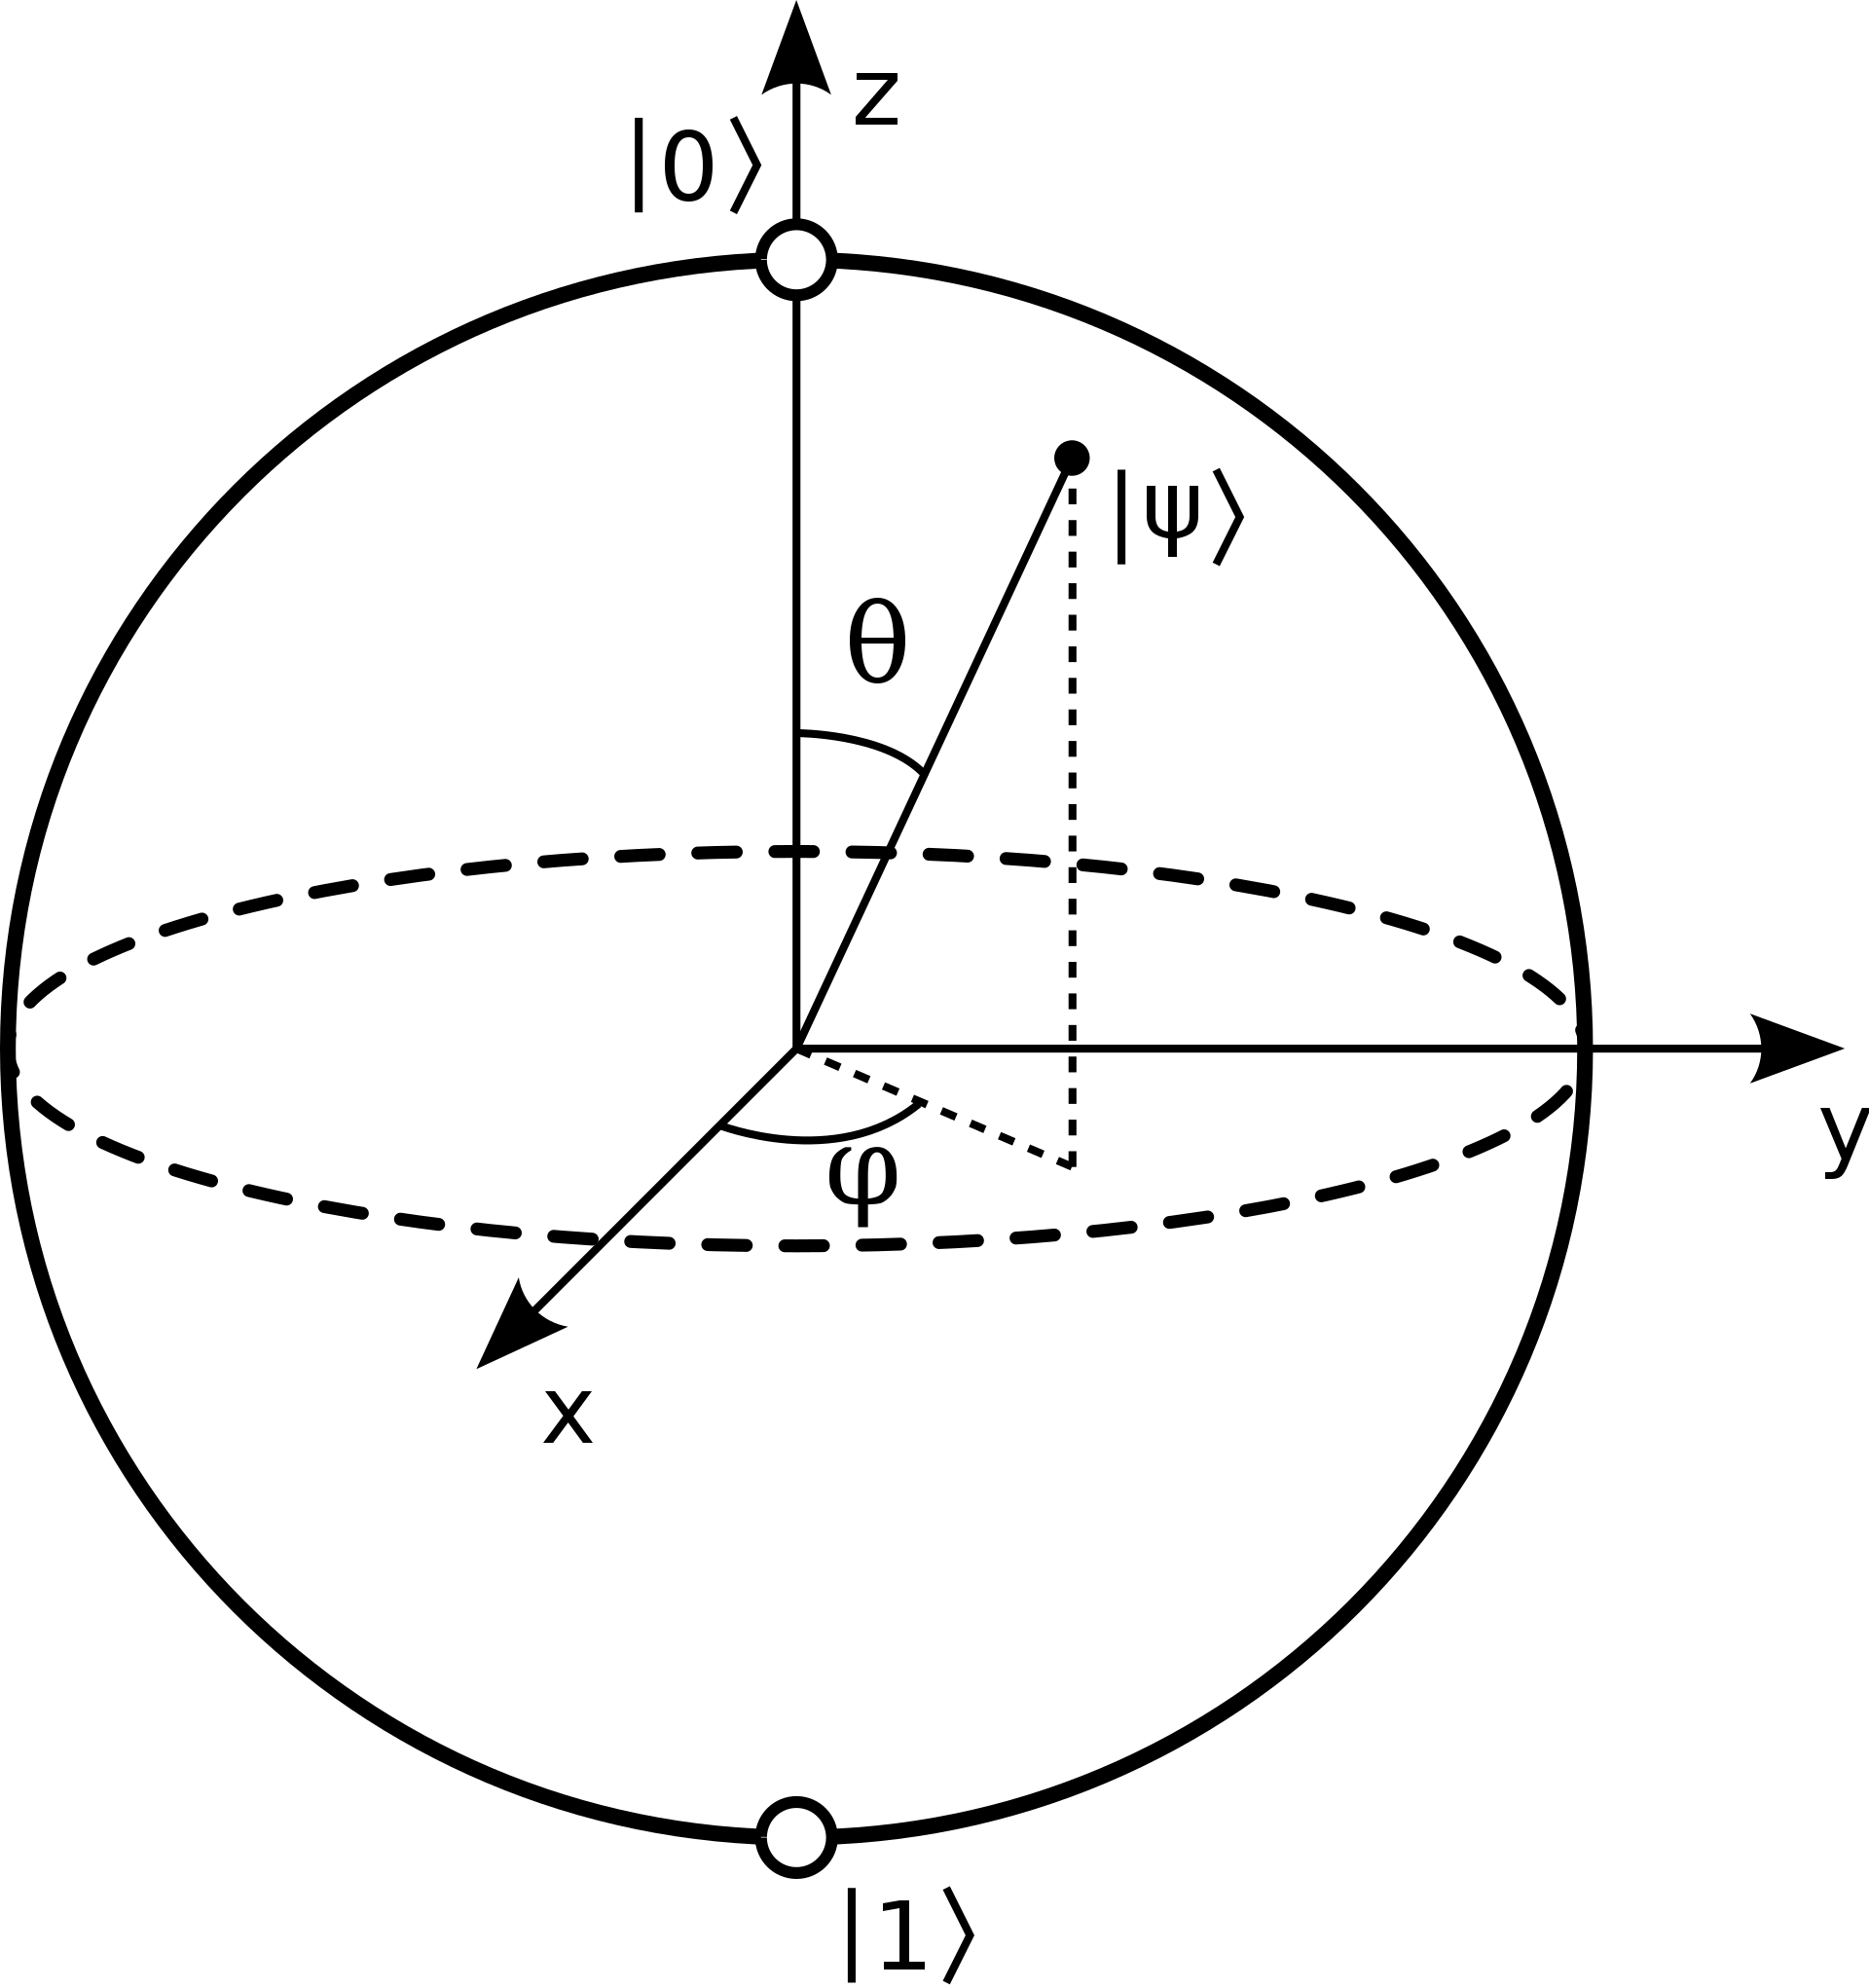
\includegraphics[scale=0.05]{bloch.png}
    \caption{$SU(2)\subseteq U(2)\cong SO(3)$.}
  \end{figure}
\end{column}
\end{columns}
\end{frame}
\begin{frame}
  \frametitle{Visualization of state sampling}
  \begin{itemize}
    \item Note that the density matrix of a single-qubit state can be expanded in the form 
    \begin{align} 
      \rho = \dfrac{1}{2}(\hat{I} +\mathbf{r}\cdot\hat{\mathbf{\sigma}}),
    \end{align}
    where $\mathbf{r}(r_x,r_y, r_z)$ is the Bloch vector, uniquely defines a mixed state. The Bloch vector component is $r_\alpha=\Tr(\sigma\cdot\rho)\in\mathbb{R}^3$.
    \item The explicit matrix representation of any arbitrary single-qubit operator $U(2)$ is 
    \begin{align}
      U(\theta,\phi,\lambda) = \begin{pmatrix}
        \cos(\theta/2) & -e^{i\lambda}\sin(\theta/2) \\
        e^{i\phi}\sin(\theta/2) & e^{i(\lambda+\phi)}\cos(\theta/2)
      \end{pmatrix},
    \end{align}
    hence each element of $U(2)$ is effectively defined by $\theta,\phi,\lambda$.
  \end{itemize}
\end{frame}
\begin{frame}
  \frametitle{Visulization of state sampling}
  \begin{columns}
    \begin{column}{0.5\textwidth}
      \begin{figure}
        \centering 
        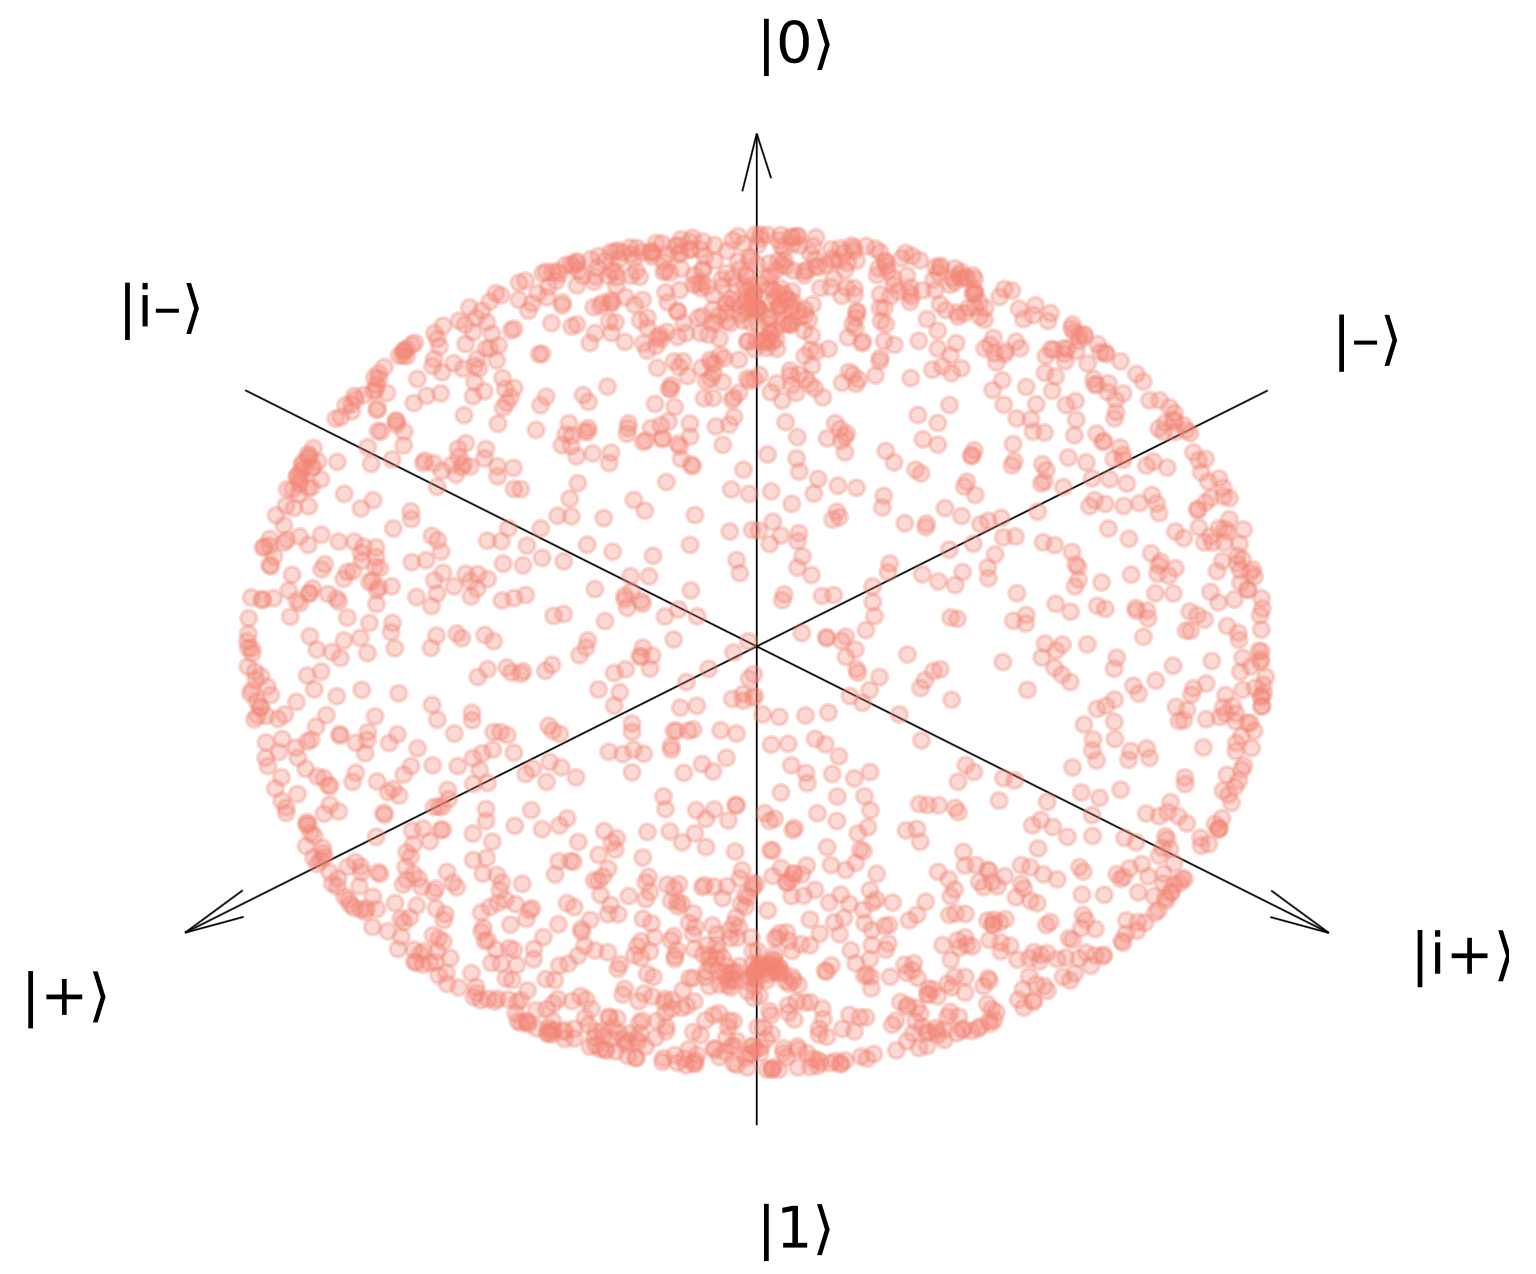
\includegraphics[scale=0.18]{bloch_not_haar.png}
        \caption{$d\mu_2=d\theta d\phi d\lambda$. Not Haar-random.}
      \end{figure}
    \end{column}
    \begin{column}{0.5\textwidth}
      \begin{figure}
        \centering 
        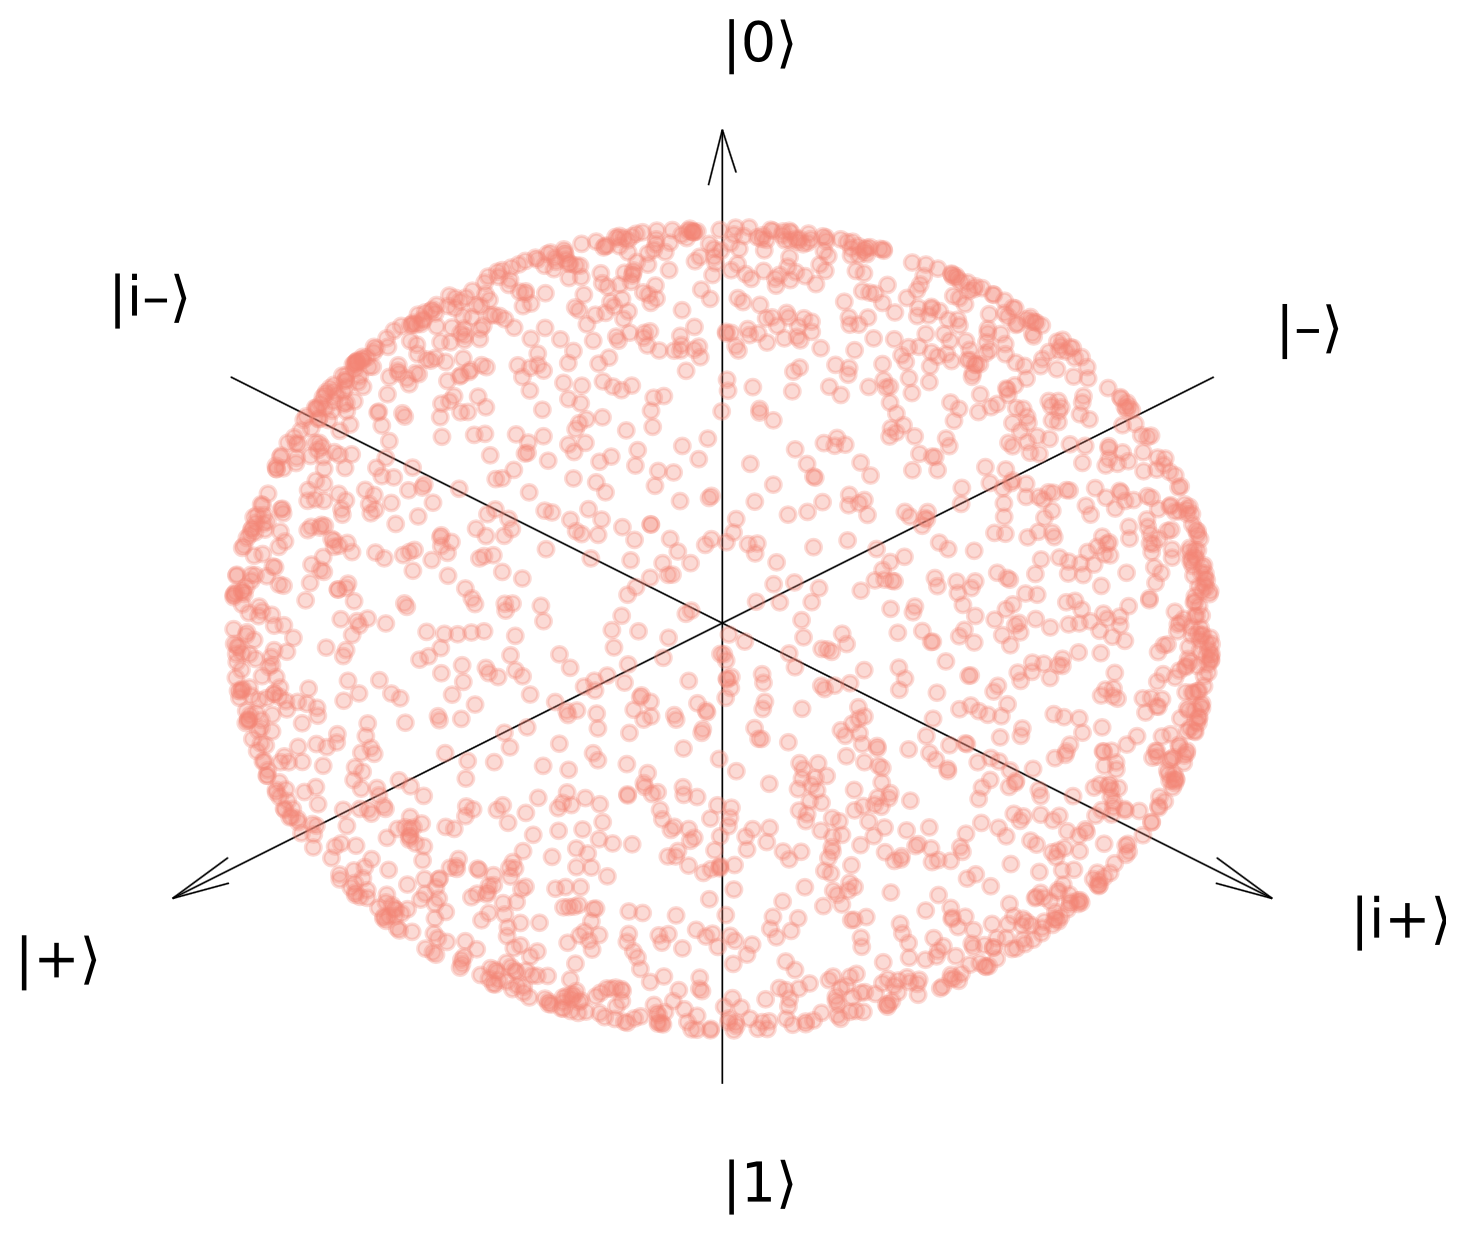
\includegraphics[scale=0.18]{bloch_haar.png}
        \caption{$d\mu_2=\sin\theta d\theta d\phi d\lambda$. Haar-random.}
      \end{figure}
    \end{column}
  \end{columns}
\end{frame}
\subsection{Haar measure in U(N)}
\begin{frame}
  \frametitle{Haar measure in $U(N)$}
  \begin{itemize}
    \item It's hard to visualize when $N=d^n$. We thus remain focus on $3^1$.
    \item From the study of photonics, we know that we can decompose any $SU(N)$ operation recursively by sandwiching an $SU(2)$ between two $SU(N-1)$ [H. de Guise \textit{et al.}, Phys. Rev. A 97 022328 (2018)].
    \item For $N=3^1$, the exact Haar measure $d\mu_3$ follows accordingly
  \end{itemize}
  \begin{figure}
    \centering
    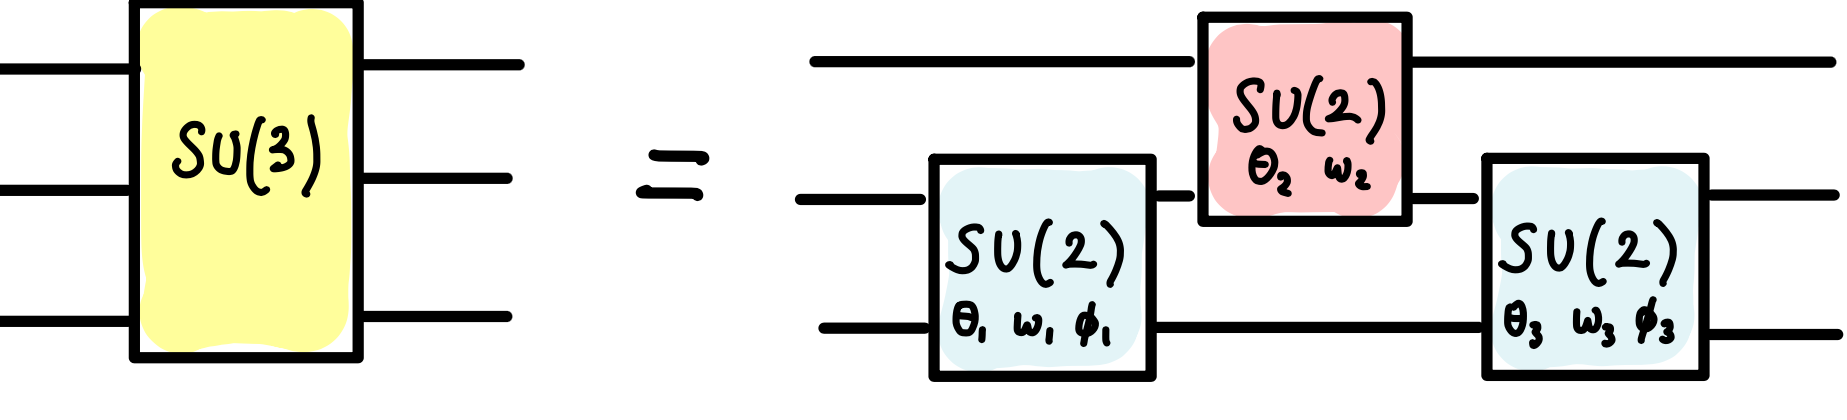
\includegraphics[scale=0.25]{su3_haar.png}
  \end{figure}
  \begin{align} 
    d\mu_3 = \sin\theta_1\sin\theta_2\sin^2(\theta_2/2)\sin\theta_3 \Pi_{i=1}^3 d\theta_i d\phi_i d\lambda_i
  \end{align}
\end{frame}
\begin{frame}
  \frametitle{Final note on Haar measure}
  \begin{itemize}
    \item Unlike $SU(2)$, sampling uniformly over $SU(3)$ requires us to sample $\theta_i$ from \textit{different distribution}.
    \item This suggests the higher dimension of the unitary group, the more parameters we need to care about. Generally speaking an $N$-dimensional unitary requires at least $N^2-1$ parameters. 
    \item Other methods of sampling uniformly are thus desired, e.g. \textit{Haar-random matrices from QR decomposition} [F. Mezzaddri, arXiv:math-ph/0609050v2 (2007)].
    \item Haar measure is invariant under unitary transformation, i.e.
    \begin{align} 
      \int_{V\in U(N)} f(WV)d\mu_N(V) &= \int_{V\in U(N)} f(VW)d\mu_N(V)\nonumber \\
      &= \int_{V\in U(N)} f(V)d\mu_N(V)\nonumber
    \end{align}
  \end{itemize}
\end{frame}
\section{Unitary t-design}
\subsection{The problem of efficient randomization} 
\begin{frame}
  \frametitle{The problem of efficient randomization}
  Sampling from $N$-dimensional unitary group requires us to keep track of $N^2-1$ parameters, or $d^{2n}-1$.
  \begin{table}[]
    \begin{tabular}{|l|l|l|l|l|l|}
    \hline
                   & 1 & 2  & 3   & $\dots$ & $n$        \\ \hline
    Qubit ($d=2$)  & 2 & 15 & 63  & $\dots$ & $2^{2n}-1$ \\ \hline
    Qutrit ($d=3$) & 8 & 80 & 728 & $\dots$ & $3^{2n}-1$ \\ \hline
    \end{tabular}
    \caption{The number of parameters we need to specify a $SU(d^n)$ operator. The exponential scaling hinders us from scalability.}
    \end{table}
    \begin{problem}[Efficient sampling]
      How to scalably and efficiently sample random unitaries in a uniform manner? 
    \end{problem}
\end{frame}
\subsection{Motivation: spherical t-design}
\begin{frame}
  \frametitle{Motivation: spherical $t$-design}
  \begin{problem}[Averaging $P$ over a sphere]
    What is the average $A$ of a $d$ variables polynomial over the surface of a real $d$-dimensional unit sphere $\mathcal{S}(R^d)$?
    \begin{align}A = \int_{\mathcal{S}(R^d)} P_t(u)d\mu(u)
    \end{align}
  \end{problem}
  \begin{itemize}
    \item This integration--in principle--can be numerically calculated, provided we have the proper measure $d\mu(u)$.
    \item What if one could alternatively approximate $A$ by uniformly sampling a sufficiently large number of points on the sphere?
    \item What if one could alternatively \textbf{calculate exactly} $A$ by uniformly sampling a sufficiently large number of points on the sphere?
  \end{itemize}
\end{frame}
\begin{frame}
  \frametitle{Motivation: spherical $t$-design}
  \begin{definition}[Spherical $t$-design]
    Let $P_t:\mathcal{S}(R^d)\rightarrow \mathbb{R}$ be a polynomial in $d$ variables with all terms homogeneous in degree at most $t$. A set $X=\{x\vert x\in\mathcal{S}(R^d)\}$ is a spherical $t$-design if 
    \begin{align} 
      \dfrac{1}{\vert X \vert} \sum_{x\in X} P_t(x) = \int_{\mathcal{S}(R^d)}P_t(u)d\mu(u) 
    \end{align}
    holds for all possible $P_t$, where $d\mu$ is the uniform, normalized spherical measure. A spherical $t$-design is also a $k$-design for all $k<t$.
  \end{definition}
  \begin{enumerate}
    \item One natural question is how do we find $X$, provided $f$?
    \item The other question concerns with the structure of the set (group) $X/\mathcal{G}$ itself.
  \end{enumerate}
\end{frame}
\subsection{Unitary t-design}
\begin{frame}
  \frametitle{Unitary $t$-design}
  Instead of averaging polynomials $P_t$ over spheres, we consider polynomials that are functions of the entries of $U\in U(N)$.
  \begin{definition}[Unitary $t$-design]
    Let $P_{t,t}(U)$ be a polynomial with homogeneous degree at most $t$ in $d$ variables in the entries of a unitary matrix $U$, and degree $t$ in the complex conjugates of those entries. A unitary $t$-design is a set of $K$ unitaries $\{U_k\}$ such that 
    \begin{align} 
      \dfrac{1}{K}\sum_{k=1}^K P_{t,t}(U_k) = \int_{U(d)} P_{t,t}(U)d\mu(U) 
    \end{align}
    holds for all possible $P_{t,t}$ and where $d\mu$ is the uniform Haar measure. 
  \end{definition}
\end{frame}
\subsection{Unitary t-design in action}
\begin{frame}
  \frametitle{Unitary $t$-design in action: Haar measure}
  Let us revisit our efficient randomization problem. The ultimate goal of randomization is to calculate the fidelity. More precisely, the \textit{average fidelity} of a quantum channel can be calculated by twirling over the Haar measure of the resprective Lie group.
  \begin{definition}[Twirling $\mathcal{E}$ over a Haar-measure]
    Suppose a quantum channel $\mathcal{E}$. The average fidelity with respect to the full set of Haar-random states $U_{\mu_N}\rho U_{\mu N}^\dagger$ is \textit{twirling channel} $\mathcal{E}$ , 
    \begin{align}
      \bar{F}_{\mathcal{E}} = \int_{U(d)} d\mu(U) U^\dagger \mathcal{E}(U\rho U^\dagger)U 
    \end{align}
  \end{definition}
\end{frame}
\begin{frame}
  \frametitle{Unitary $t$-design in action: Fidelity}
  Using the result of [J. Emerson \textit{et al.}, arXiv:quant-ph/0606161v2 (2012)], we conclude that twirling any quantum channel over a unitary $t$-design is equivalent to twirling over a Haar-measure unitary group.
  \begin{align}
    \dfrac{1}{K}\sum_{j=1}^K U_j^\dagger \mathcal{E}(U_j\rho) U_j = \int_{U(d)} d\mu(U) U^\dagger \mathcal{E}(U\rho U^\dagger)U 
  \end{align}
  \begin{itemize}
    \item Note that the inner product involves two $U$ and two $U^\dagger$, thus implies this unitary $t$-design is a \textit{unitary 2-design}.
    \item What is the unitary 2-design then?
  \end{itemize}
\end{frame}
\begin{frame}
  \frametitle{Twirling over Clifford group}
  \begin{theorem}[$\mathcal{C}^n_3$]
    The multi-qutrit Clifford group $\mathcal{C}^n_3$ forms a unitary 2-design.
  \end{theorem}
  A result from [M. Nielsen, arXiv:quant-ph/0205035v2 (2002)] prove that twirling a quantum channel $\mathcal{E}$ over a Haar measure yields a depolarizing channel.
  \begin{corollary}
    Twirling over the multi-qutrit Clifford group yields a depolarizing channel.
  \end{corollary}
  From this, we informally confirm the aformentioned results of URB,
  \begin{align} 
    \mathcal{E}_{dep}(\rho_i) = p\rho_i + (1-p)\dfrac{I}{3^n}
  \end{align}
\end{frame}
\section{Conclusion}
\begin{frame}
  \frametitle{Conclusion}
  \begin{enumerate}
    \item The metrics we concern is the average fidelity of a quantum channel $\mathcal{E}$. This average fidelity can be calculated by twirling that channel over Haar-random unitary group [J. Emerson \textit{et al.}, arXiv.quan-ph/0503243].
    \item This is better than QPT, but still not scalable and efficient. We can however get around by using the unitary $t$-design. 
    \item Twirling over a unitary $t$-design is equivalent to twirling over Haar-random unitary group, and yields a depolarizing channel.
    \item The depolarizing channel has an exponential decay with respect to gate length $m$. 
  \end{enumerate}
  Next week: The Clifford group $\mathcal{C}_3$ on single-qutrit.

\end{frame}
\end{document}